\section{Dataset} \label{sec:dataset}
Our primary source of data is automatic data capture from TTNet \cite{voeikov2020ttnet}, as released by OSAI \cite{OSAI}. We use their Tokyo 2020 Olympics and Tischtennis-Bundesliga (German table tennis league) sets, which include men and women's singles matches and player statistics. Many potential features such as player age, rank, match duration as well as in-match statistics such as percentage of points won on serve and receive, stroke types and error types are available. Interactive maps that demonstrated the ball position of each shot on the table, as well as the stroke type were also accessible. The progression of a rally and location of each ball bounce can be mapped into a sequence (see \figref{sequence}).

%\denes{Can we say that one of the challenges is to find out which features might be salient for a result predictor?}

\begin{figure}[t]
\centering

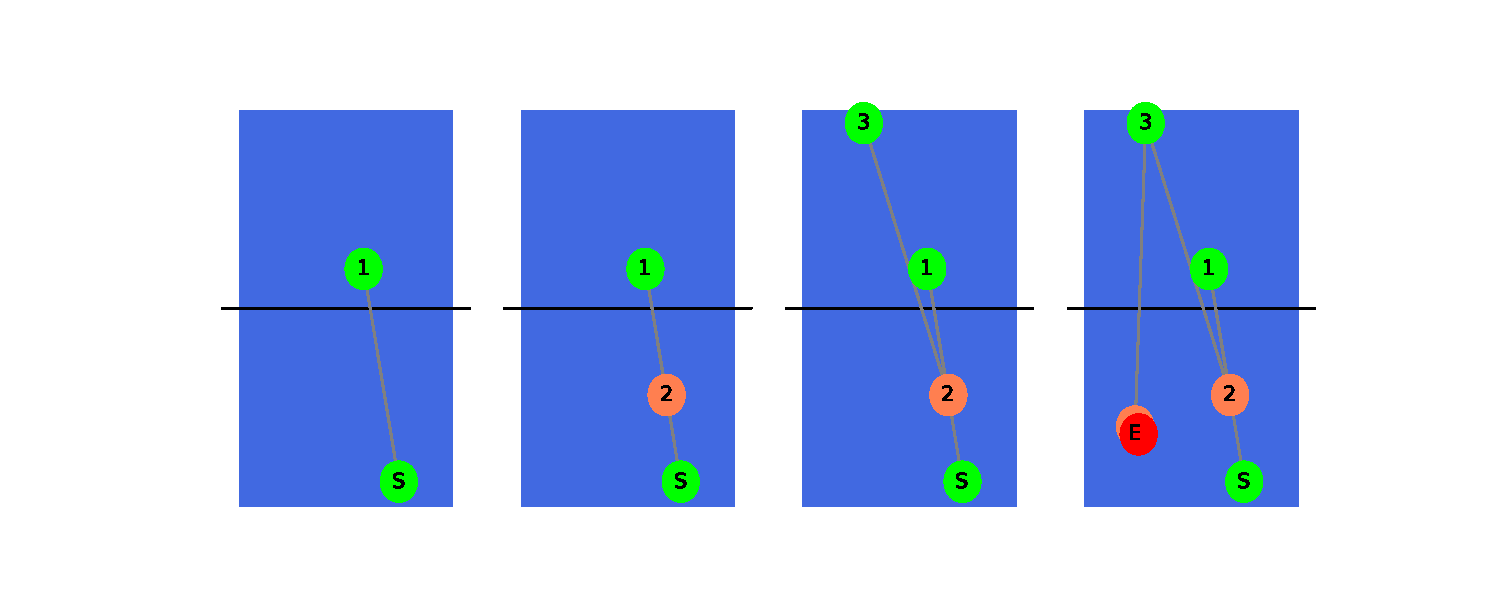
\includegraphics[width=8.5cm]{plots/tablesequence.pdf}
\caption{Progression of a rally demonstrating the landing point of each ball bounce. Yellow indicates service which starts a rally and red indicates an error ending the rally. Green indicates all other ball bounces \cite{OSAI}.}
%\denes{Please remove all margins on these plots}}

\label{fig:sequence}
\end{figure}

As the sequence of co-ordinates is not always intuitive to interpret, the whole rally can be instead reduced to the location of the winning shot. Furthermore, each half of the table can be split into nine equal sections, and the location of every winning shot of the match can be grouped into one of these parts (\figref{pos}). Further grouping can involve the number of forehands and the number of backhands used to win a point (\figref{fvbh}), or whether it was 'short` or 'long` rally (\figref{svlr}). We use this data to measure the strength of different skills of a player in different aspects of the sport. \denes{which version? Fig 3 or 4?}. Samples with missing data entries were removed from the dataset.

\begin{figure}[t]
\centering

%\vspace{-2em}
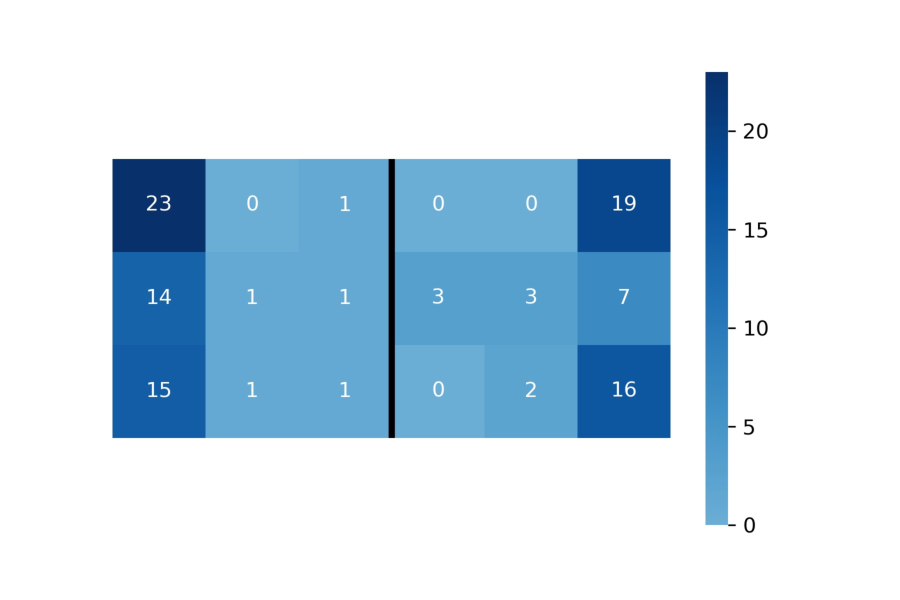
\includegraphics[width=8cm]{plots/tableheatmaplot.pdf}
\caption{Distribution of ball placement of a winning shot for both players by region if each side of the table were to be split into nine equal parts. Each value indicates the number of balls landing in it's respective region \cite{OSAI}.}

\label{fig:pos}
\end{figure}



\begin{figure}[ht]
\centering

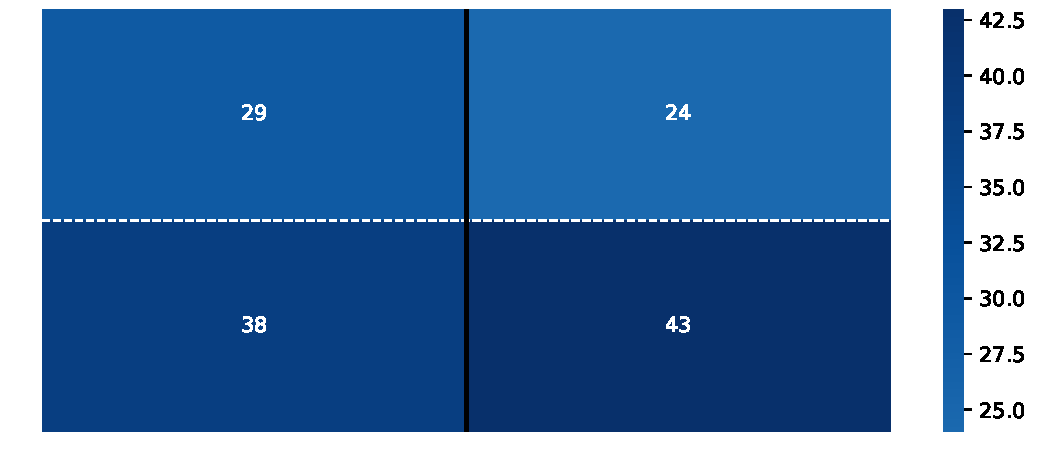
\includegraphics[width=8cm]{plots/forehandvsbackhand.pdf}
\caption{Distribution of points won by forehand compared to a backhand \cite{OSAI}.}

\label{fig:fvbh}
\end{figure}

\begin{figure}[ht]
\centering

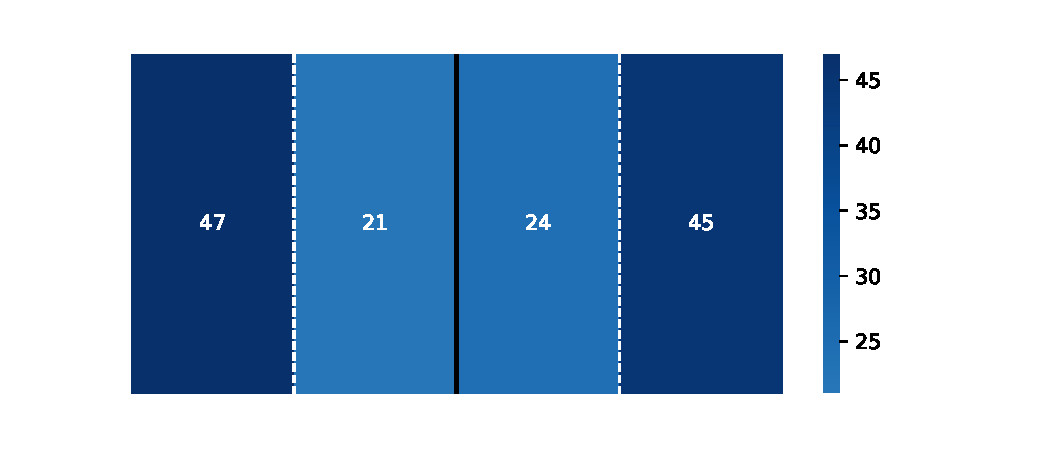
\includegraphics[width=8cm]{plots/shortvslongrally.pdf}
\caption{Distribution of points won by a short rather than long rally \cite{OSAI}.}

\label{fig:svlr}
\end{figure}


 
 %One of the main challenges in constructing a successful result predictor is the selection of salient features. To address this, we carefully hand picked features that we thought would be the most influential in a match based on existing domain knowledge on the problem.